%% beamerthemeImperialPoster v1.0 2016/10/01
%% Beamer poster theme created for Imperial College by LianTze Lim (Overleaf)
%% LICENSE: LPPL 1.3
%%
%% This is the example poster demonstrating use
%% of the Imperial College Beamer Poster Theme
\documentclass[xcolor={table}]{beamer}
%% Possible paper sizes: a0, a0b, a1, a2, a3, a4 (although Imperial College posters are usually A0 or A1).
%% Possible orientations: portrait, landscape
%% Font sizes can be changed using the scale option.
\usepackage[size=a0,orientation=portrait,scale=1.55]{beamerposter}

\usetheme{CBBLPoster}

%% Four available colour themes
\usecolortheme{CBBLWhite} % Default
% \usecolortheme{CBBLLightBlue}
% \usecolortheme{CBBLDarkBlue}
% \usecolortheme{CBBLBlack}

\title{A Bioinformatics Pipeline Reveals a Shared I$\kappa$B$\alpha$ Interface for NF-$\kappa$B  and Histone Binding}
\author{Martin Floor\Tsup{1,3}, \mainauthor{Jordi Villà-Freixa}\Tsup{1,2}, Joan Bertran\Tsup{1,2} and Lluís Espinosa\Tsup{4}}

\institute{\Tsup{1}Computational Biochemistry and Biophysics Lab, Faculty of Sciences, Engineering and Technology, Universitat de Vic - Universitat Central de Catalunya\\\Tsup{2}Institut de Recerca i Innovació en Ciències de la Vida i de la Salut a la Catalunya Central\\\Tsup{3}Barcelona Supercomputing Center, Life Sciences Department\\\Tsup{4}Hospital del Mar Research Center}

\addbibresource{JBI2025_FEEC.bib}


\begin{document}
\begin{frame}[fragile=singleslide,t]\centering

\maketitle

\begin{block}{Summary}
I$\kappa$B$\alpha$, traditionally a negative regulator of NF--$\kappa$B, has recently been linked to chromatin-dependent transcriptional control\citep{Marruecos2021}. 
We developed a bioinformatics pipeline to identify conserved, surface-exposed residues mediating protein interactions. 
Our Fold-Excluded Evolutionary Conservation (FEEC) metric integrates structural packing (WCN) and evolutionary conservation (ConSurf) to prioritize I$\kappa$B$\alpha$ binding residues. 
FEEC highlighted an ANK-repeat surface engaging both the $p65$ NLS and histone H4 tail. 
Guided by FEEC, we engineered separation-of-function (SOF) mutants disrupting either NF--$\kappa$B binding (SOF$^{\Delta\mathrm{NF}\text{-}\kappa\mathrm{B}}$) or histone association (SOF$^{\Delta\mathrm{H2A/H4}}$). 
Structural modeling, mutagenesis, and functional assays confirmed their specificity. 
Transcriptomic analysis of SOF$^{\Delta\mathrm{NF}\text{-}\kappa\mathrm{B}}$ cells revealed repression of intestinal stem-cell genes independent of NF--$\kappa$B, underscoring a chromatin-related role for I$\kappa$B$\alpha$. 
FEEC thus provides a generalizable framework to resolve multifunctional protein interfaces.\citep{Alvarez-Villanueva2025}

\end{block}

\begin{columns}[onlytextwidth,T]

%%%% First Column
\begin{column}{.47\textwidth}


\begin{figure}
    \centering
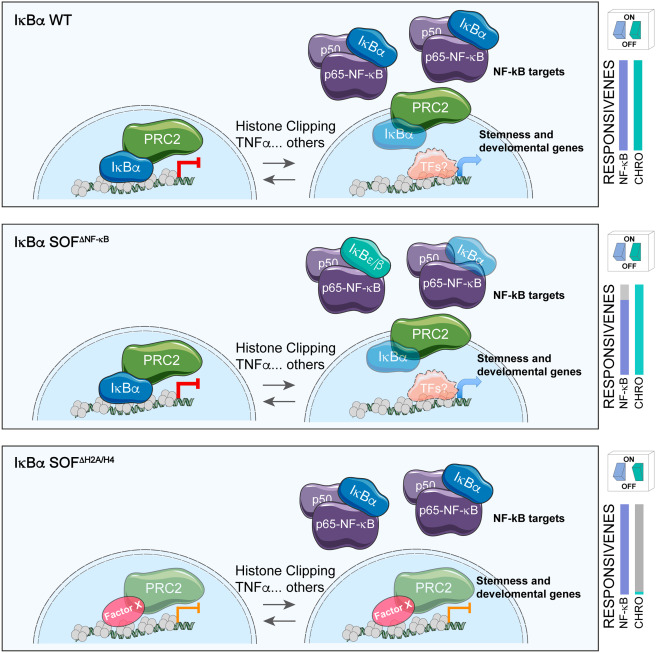
\includegraphics[width=0.7\linewidth]{SOF_summary.jpg}
\caption{Regulation of NF-$\kappa$B and PRC2 target genes by I$\kappa$B$\alpha$ WT and SOF mutants}
\end{figure}


\begin{block}{Methodology}
\section*{Method Details}

The \textbf{Weighted Contact Number (WCN)} quantifies atomic contact density from interatomic deistances as
\[
\mathrm{WCN}_i = \sum_{j \neq i} \frac{1}{r_{ij}^2}, \quad
\mathrm{iWCN}_i = \frac{1}{\mathrm{WCN}_i}.
\]
Sequence conservation scores (\(S_{C,i}\)) were obtained from the \textsc{Consurf} server and expressed as Z-scores. The \textbf{Fold-Excluded Evolutionary Conservation (FEEC)} score identifies residues with conservation beyond structural constraints:
\[
\mathrm{FEEC}_i = \mathrm{iWCN}_i - S_{C,i}.
\]
Interface energies were computed from Rosetta-generated conformations weighted by Boltzmann probabilities and expected bingin energies:
\[
P_i = \frac{e^{-E_i/kT}}{\sum_{i=1}^N e^{-E_i/kT}},
\]
\[
\langle E_{\text{binding}} \rangle = \sum_i P_i E_{b,i}, \quad E_{b,i} = E_{\text{complex},i} - (E_{A,i} + E_{B,i}).
\]
Mutational effects were estimated after repacking and minimizing residues within 8\,\AA\ of each mutation site.
\end{block}

\end{column}


%%%% Second Column
\begin{column}{.47\textwidth}
\begin{block}{Common domain of I$\kappa$B$\alpha$ binding to p65-NF-$\kappa$B and H2A/H4}
FEEC scores accurately predicted most I$\kappa$B$\alpha$/NF-$\kappa$B interface residues (83\% for p65, 73\% for p50), validating FEEC as a reliable predictor of binding sites.
Mapping positive FEEC residues revealed strong overlap with known interface regions from structural data.
Negatively charged FEEC-positive residues in the ANK1-ANK2 domains (e.g., D73, D75, E85, E86) likely form the binding site for the histone H4 N-terminal tail, overlapping with the p65-NF-$\kappa$B NLS interaction region.
\begin{figure}
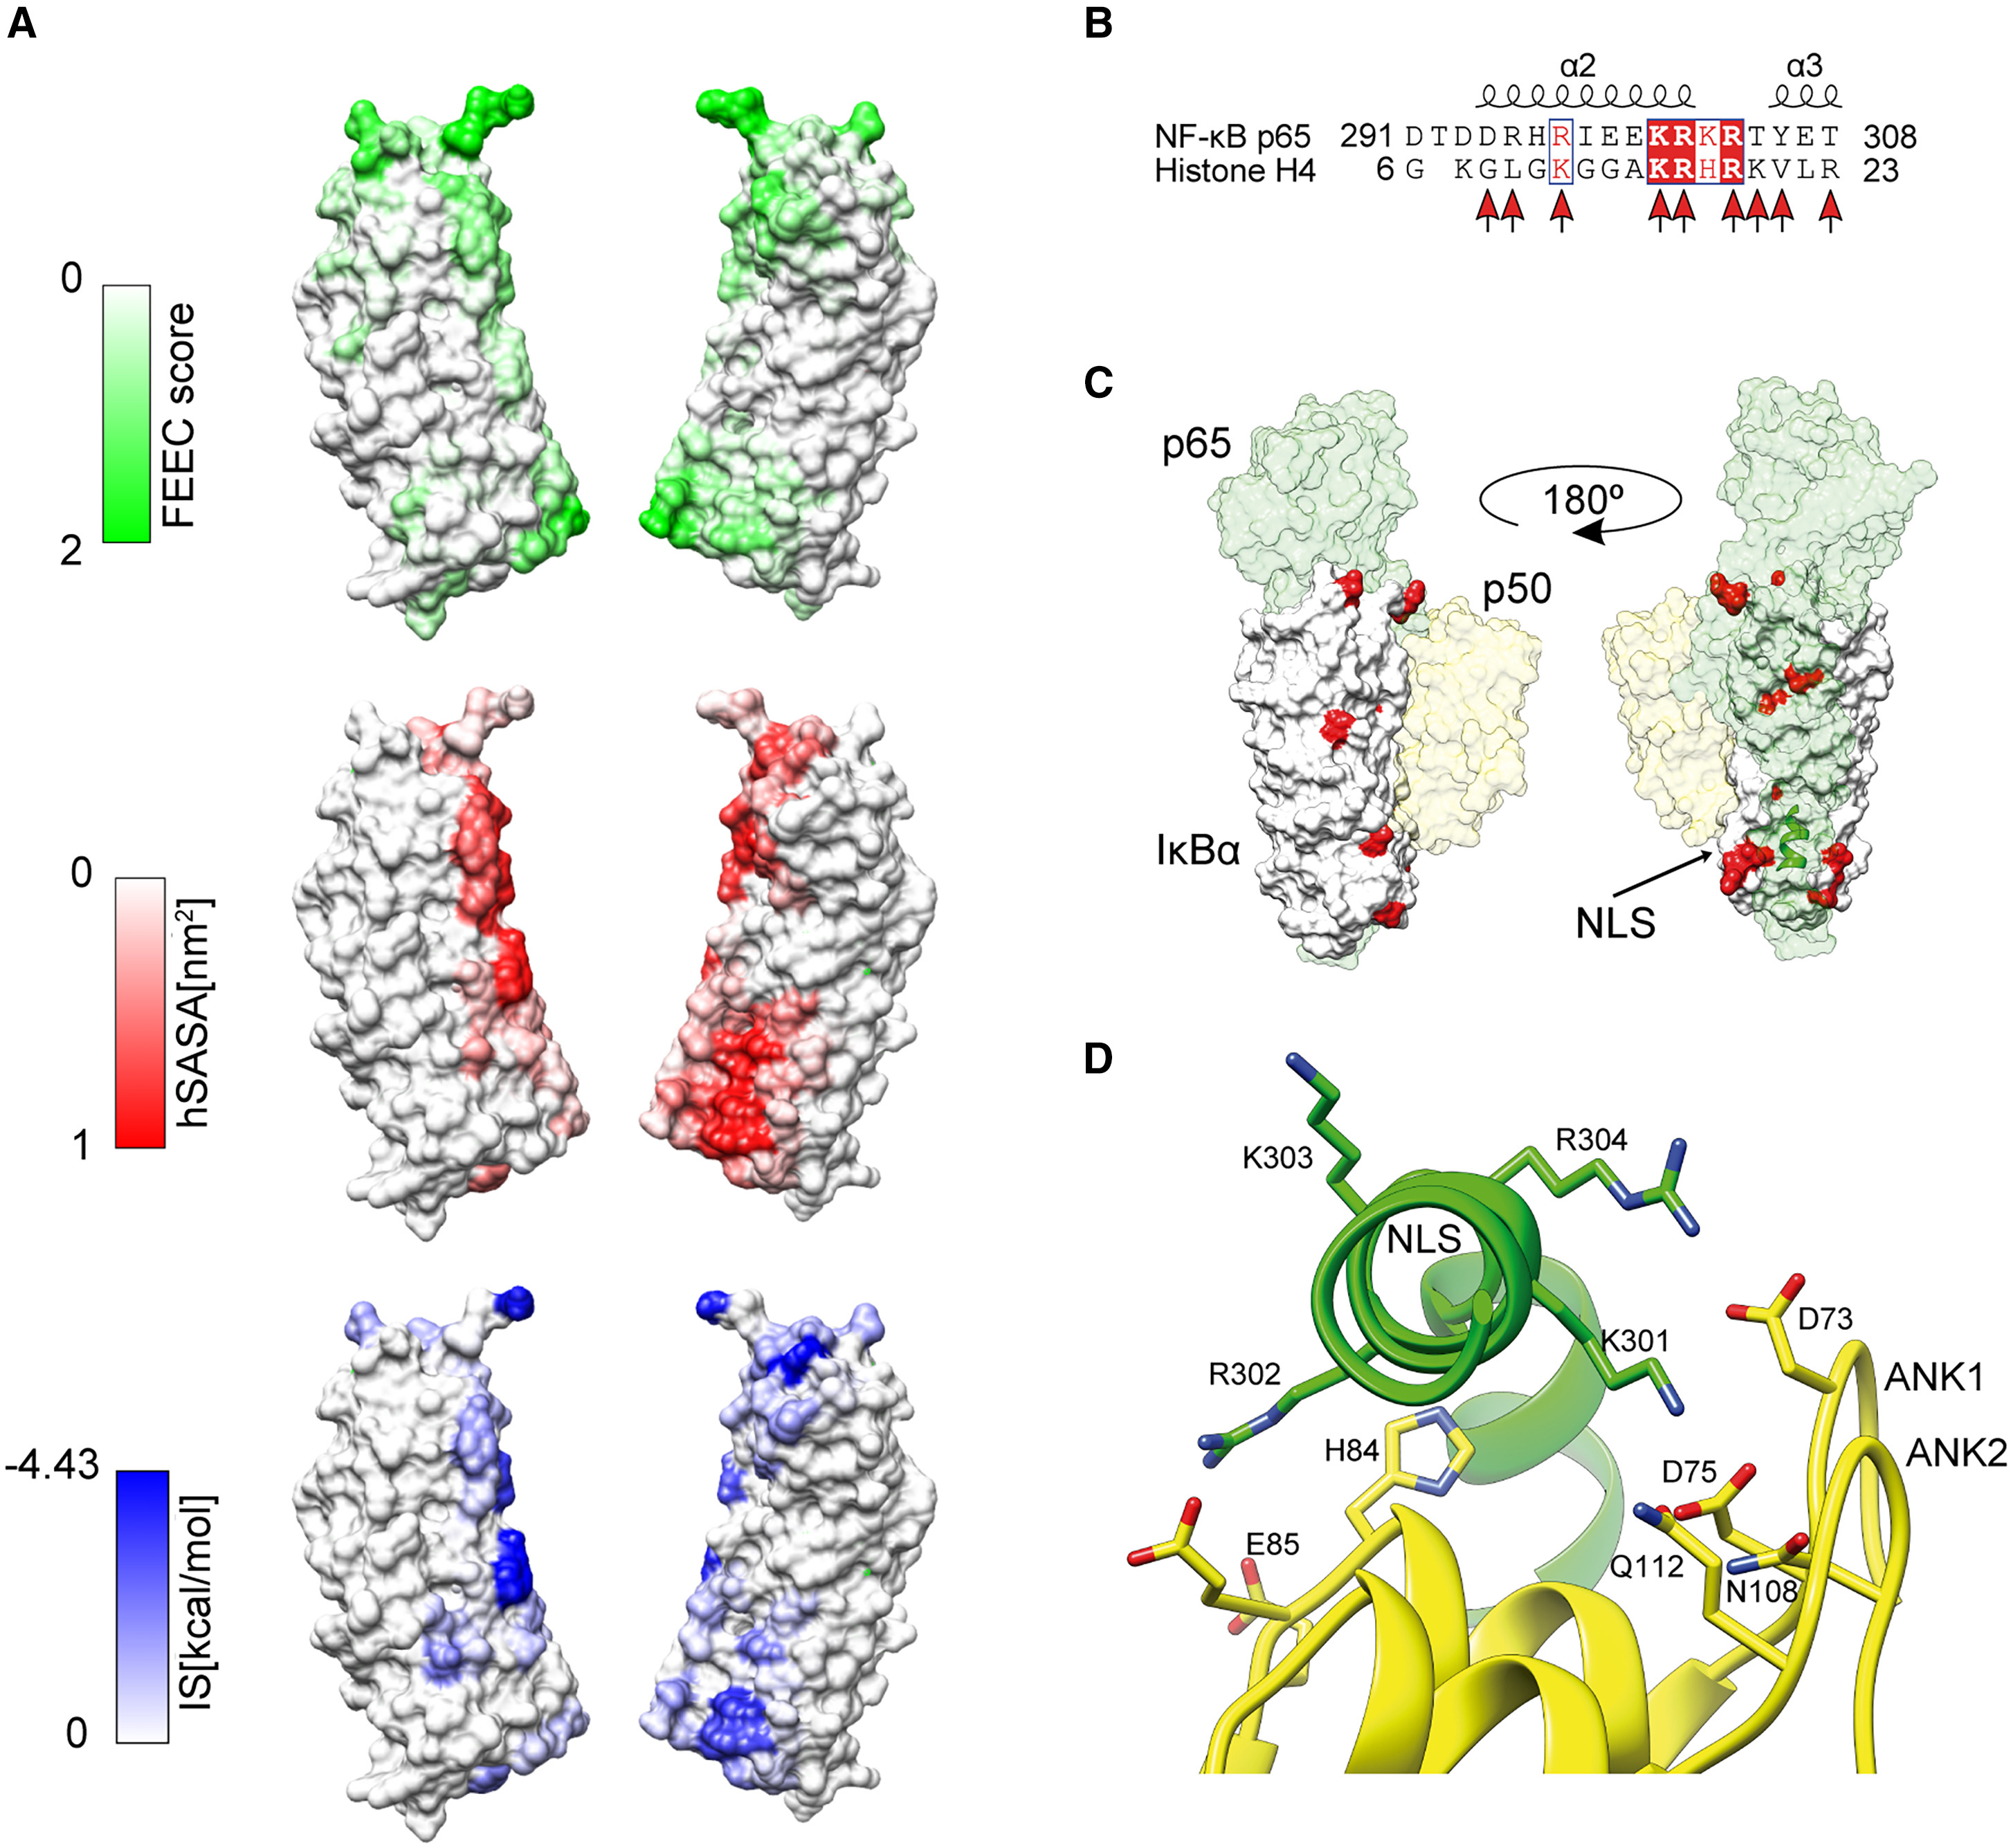
\includegraphics[width=\hsize]{SOF_FEEC.jpg}
\caption{(A) Surface mapping of I$\kappa$B$\alpha$ residues with positive FEEC scores (capped at 2), solvent-accessible area buried upon NF--$\kappa$B binding, and per-residue interface scores (PDB: 1NFI). 
(B) Alignment of the p65-NF--$\kappa$B NLS region with the H4 N-terminal tail; conserved positions (blue), similar/identical residues (red/white), and I$\kappa$B$\alpha$-contacting residues (red arrows) are indicated (PDB: 3UW9). 
(C) I$\kappa$B$\alpha$ (white)-NF--$\kappa$B (p65, green; p50, yellow) complex showing negatively charged I$\kappa$B$\alpha$ residues with FEEC>0  (red). 
(D) Interaction of the p65 NLS motif (KRKR, green) with I$\kappa$B$\alpha$ ANK1-2 repeats; polar interacting residues in yellow. UniProt Q04206 (p65) and P25963 (I$\kappa$B$\alpha$).}
\end{figure}
\end{block}
\end{column}
\end{columns}
 \vspace{-1ex}% 
\printbibliography
\end{frame}
\end{document}